\subsubsection{Minuta de reunião (15-Julho-2015)}

\begin{tabbing}
  Local \= xxx \kill
  Local \> : LEAD \\
  Data  \> : 15 de Julho de 2015 \\
  Hora  \> : 13:00
\end{tabbing}

%---------------------------------------------------------------------
\participantes{
  \elael,
  \alana,
  \gabriel,
  \julia,
  \ramon,
  \renan.
}

\textbf{Aprovação da minuta}

\textbf{Update semanal do Projeto EMMA}

  
\textbf{\renan.} 
	\begin{itemize}
		\item \textbf{Tarefas concluídas:}
			\begin{itemize}    
				\item Repasse do relatório da viagema Rijeza.
			\end{itemize}
		
		\item \textbf{Novas tarefas:}
			\begin{itemize} 
				\item Dar continuidade a análise de pás com Estevão.
				\item Formalizar descobertas de Porto Alegre, e dar início a um novo
				Journal.
				\item Descobrir com Ramon onde publicar o artigo.
			\end{itemize}
	\end{itemize}
		
\textbf{\elael.} 
	\begin{itemize}
		\item \textbf{Tarefas concluídas:}
			\begin{itemize}    
				\item Pesquisa de Sensores.
			\end{itemize}
		
		\item \textbf{Novas tarefas:}
			\begin{itemize} 
				\item Formalizar Pesquisa de Sensores.
			\end{itemize}
	\end{itemize}
					
			
   \textbf{\gabriel.} 
	\begin{itemize}
		\item \textbf{Tarefas concluídas:}
			\begin{itemize}    
				\item Formalizou pesquisa de Sensores de alta precisão com pros e cons:
				Pros: sensores não são 3d e sim fechos de laser com um espelho giratório e
				um PanTilt que varre o ambiente.
				Cons: Tais sensores demoram muito para fazer a varredura completa.
			\end{itemize}
		
	\end{itemize}

			
\textbf{\estevão.} 
	\begin{itemize}
		\item \textbf{Tarefas concluídas:}
			\begin{itemize}    
				\item Metodologia criada: malha de pontos, rotina que identifica o
				manipulador específico que atende aos parâmetros do projeto. Os
				manipuladores pesquisados estão sendo adicionados de acordo.
				\item Análise cinemática e dinâmica com OpenRave e MathLab para simulação
				dinâmica.
			\end{itemize}
		
		\item \textbf{Novas tarefas:}
			\begin{itemize} 
				\item Produzor gráfico para pá robótica.
				\item Maquete de braço.
				\item Opções de estagiário.
			\end{itemize}
	\end{itemize}
	
		
   \textbf{\julia.} 
	\begin{itemize}
		\item \textbf{Tarefas concluídas:}
			\begin{itemize}    
				\item Fluxograma com tarefas do robô descritas
			    \item Estudo de artigos para pesquisa de mapping e visualização de data.
			\end{itemize}
		
		\item \textbf{Novas tarefas:}
			\begin{itemize} 
			 \item Fluxograma Macro
			 \item Formalizar pesquisa de Mapping.
			 \item entregar proposta revisada
			\end{itemize}
	\end{itemize}

			



\textbf{Agenda para a próxima reunião:}
  \begin{itemize}
    \item Resultado de pesquisas individuais.
    \item Novas tarefas \& recomendações.
  \end{itemize}


\vspace{5mm}%
\parbox[t]{70mm}{
  Aprovado por: \\[5mm]
  \centering
  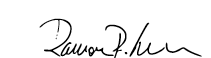
\includegraphics[width=65mm]{figs/logo/assinatura-ramon.png} \\[-4mm]
  \rule[2mm]{70mm}{0.1mm} \\
  \ramon \\[1mm]
  Coordenador do Projeto \\
}

%---------------------------------------------------------------------
\fim